\begin{figure}[!htb]
\begin{center}
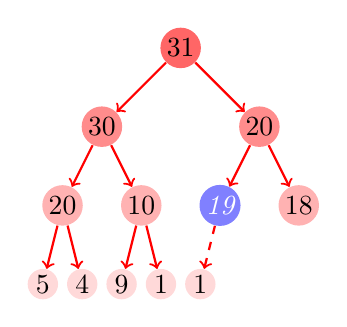
\begin{tikzpicture}
[
	xscale	= 1,	% to scale horizontally everything but the text
	yscale	= 1,	% to scale vertically everything but the text
	%
	%
	% ----------- options for the tree --------------
	level distance	= 10mm,
	%
	every node/.style =
	{
		fill		= red!60,
		circle,
		inner sep	= 1pt
	},
	%
	level 1/.style =
	{
		sibling distance	= 20mm,
		nodes				= {fill=red!45}
	},
	%
	level 2/.style =
	{
		sibling distance	= 10mm,
		nodes				= {fill=red!30}
	},
	%
	level 3/.style =
	{
		sibling distance	= 5mm,
		nodes				= {fill=red!15}
	},
	%
	edge from parent/.style =
	{
		draw,
		red,
		thick,
		->
	}
]



% actual tree
\node {31}
child
{
	node {30}
	child
	{
		node {20}
		child
		{
			node {5}
		}
		child
		{
			node {4}
		}
	}
	child
	{
		node {10}
		child
		{
			node {9}
		}
		child
		{
			node {1}
		}
	}
}
child
{
	node {20}
	child
	{
		node [color = blue!50, text = white, font = \itshape] {19}
		child
		{
			node {1}
			edge from parent [dashed]
		}
		child[missing]
	}
	child
	{
		node {18}
	}
};





\end{tikzpicture}
%
\caption{A more complicated example of a tree, with also modified links.}
\label{fig:trees__modifying_the_links}
%
\end{center}
\end{figure}

